\section{Domain Analysis of \hpl}
\label{sec:domainAnalysis}

Although tailored to managing variability in a specific SPL~\cite{ferreira:2010}, some users of Hephaestus
would appreciate more specific configurations of the
tool. For instance, some users could be interested in managing
variability only in requirements and use cases; others could be
interested in managing variability only in source code; and yet other
engineers could be interested in managing variabilities in
requirements, use cases, and source code.
Accordingly, new extensions of Hephaestus have been recently proposed. For
instance, currently there are variants of Hephaestus supporting variability in business
processes models~\cite{Machado:2011:MVB:1960502.1960508} and \emph{Simulink} assets~\cite{simulink}.

These variants share the same configurability and flexibility issues explained in Section~\ref{sec:hephaestus}. To address these issues, we adopt a SPL perspective to Hephaestus itself, thus leveraging the commonality in these variants and systematically managing the incurred variability. Since there are existing versions of Hephaestus, we adopt the extractive strategy~\cite{kruegerPFE01}, bootstrapping the Hephaestus-PL from such variants. Correspondingly, we  analyzed the existing variants of \hp{} and manually identified the common and variable features, architectural and implementation elements. The remainder of this section explains the result of this strategy to identify commonality and variability among such elements. In Section~\ref{sec:domainDesign}, we present and explain how \hpl's domain design leverages this domain analysis and addresses configurability and flexibility; the details of implementation are presented in the Section~\ref{sec:implementation}. Section~\ref{sec:process} details the reactive process needed to introduce support for managing variabilities in new assets flexibly.

\subsection{\hpl's Feature Model} \label{feature-model-hpl}

In terms of problem space, Hephaestus-PL' feature model is represented in Figure~\ref{fig:hephaestus-fm-03}. As
the diagram shows, the \emph{SPLAsset} feature is mandatory and \emph{OutputFormat} feature is optional and are
parents of \emph{or-features} so that any combination of models and output formats are
supported, e.g., a given instance might comprise business processes and use cases and export both
assets as XML files. Managing variabilities in such a combination of features is essential in \hpl{} and
has not been addressed in related work (Section~\ref{related-work} discusses this).

In addition to the feature diagram, Figure~\ref{fig:hephaestus-fm-03} shows some cross tree constraints that must be satisfied for any valid feature configuration of Hephaestus-PL. 
To illustrate, Figures~\ref{fig:hephaestus-conf1a} and~\ref{fig:hephaestus-conf1b} show two valid configurations of Hephaestus-PL, whereas Figure~\ref{fig:hephaestus-conf-invalid} shows an invalid configuration of Hephaestus-PL, in which
the \emph{UcmToXML} feature is selected, but the \emph{UseCase} feature is not selected. In this case,
the $UcmToXML \lor UcmToLatex \rightarrow Use Case$ constraint was violated, leading to an invalid feature
configuration of Hephaestus-PL.


\begin{figure*}[htb]
\begin{center}
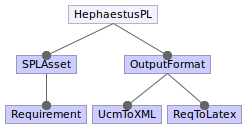
\includegraphics[scale=0.6]{imagens/confInvalid.png}
\end{center}
\caption{\hpl's invalid configuration}
\label{fig:hephaestus-conf-invalid}
\end{figure*}

% slide 8




\begin{figure*}[bth]
\begin{center}
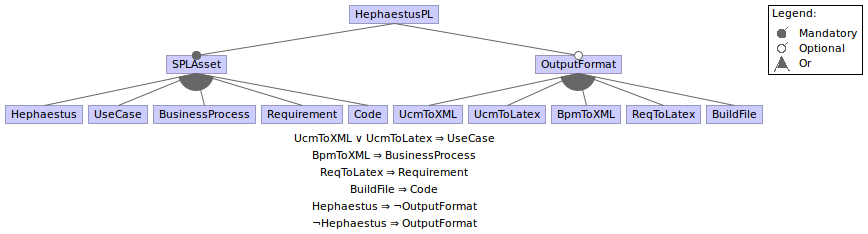
\includegraphics[scale=0.5]{imagens/fm-hpl.png}
\end{center}
\caption{\hpl's feature model. In this version, the features \textit{SPLAsset} and \textit{OutputFormat}
  define an \emph{or} relationship with their children}
\label{fig:hephaestus-fm-03}
\end{figure*}





\subsection{\hpl's Commonality and Variability} \label{domain-analysis-hpl}
%@vra: address mention to related work below

In the solution space, there exists significant amount of commonality among these versions: the \texttt{build} function as well as other supporting functions and data types are shared among all such variants of Hephaestus.  On the other hand, variability has regular form requiring both
open data types and open functions, as explained in Section~\ref{hp-evolution}. In particular, the result of the domain analysis is consistent with the evolution history reported previously and revealed that commonality resides in the following:

\begin{itemize}
  \item product configuration representation: an algebraic data type represents a valid feature configuration.

  \item feature model representation: an algebraic data type represents the feature model of a product line.

  \item basic CK representation: an algebraic data type represents the product line's  \texttt{ConfigurationKnowledge}.

  \item product instantiation: the \texttt{build} function performs the SPL instantiation by generating a product corresponding to a specific product line configuration.


\end{itemize}

On the other hand, our domain analysis revealed that \hpl{} variability resides in the following:

\begin{itemize}
  \item \textbf{Asset Representation}: algebraic data types represent the abstract syntax of different SPL assets (such as use cases, business processes, and code).

  \item \textbf{Asset Transformations}: functions manipulate such artifacts, solving variability of SPL assets. Some transformations
  basically select a specific asset from the product line, including it into the product during product derivation. Other transformations
  change the structure of an asset of the SPL in the final product.

  \item \textbf{Asset IO}: parser/output functions for reading/writing artifacts convert the concrete syntax of an asset to/from the corresponding
  abstract syntax of \hpl{}, i.e., the asset abstract data types.

  \item \textbf{Asset Wrapping}: the \texttt{SPLModel} and \texttt{InstanceModel} algebraic data types comprise the set of SPL assets and the feature model (feature configuration in case of \texttt{InstanceModel}) field of a given \hpl{} instance.

  \item \textbf{Empty Instance}: defines the initial representation of a product
  during the product derivation activity. It is an instance of the \texttt{InstanceModel} data type and serves
  as a baseline that is successively refined by the \texttt{build} function (see Figure~\ref{fig:spl-model-with-req-and-code})
  until all appropriate transformations have been applied and the final product derived.

%  \item \texttt{exportProduct} function: is the function that exports a derived product. Usually, this function calls
%   several \emph{output functions} to export the final product.

  \item \textbf{CK's parser} (\texttt{xml2Transformation} function): it does the recognition of the concrete syntax of
   transformations to populate the asset's CK.

\end{itemize}

Although at the domain level a specific configuration of Hephaestus represented by the combination of \textit{or-features} is conceptually simple, in the solution space it is more complex because it represents managing variability in a combination of artifacts at different levels of granularity (i.e., course-grained and fine-grained), and the implementation of the features preserves some degree of scattering and tangling in Hephaestus' source code.
For example, to introduce variability support for one new asset in Hephaestus, we had to implement the
data types for representing the abstract syntax of these models, implement the transformations for solving variability,
implement the parser and output functions for reading/writing these assets into/from Hephaestus, and we had to extend some data types and functions of Hephaestus (as detailed in Section~\ref{hp-evolution}).




